\documentclass[11pt]{article}
\usepackage[margin=1in]{geometry}
\usepackage{amsmath,amssymb}
\usepackage{listings}
\usepackage{xcolor}
\usepackage{tikz}
\usetikzlibrary{arrows.meta,positioning,fit,calc}
\usepackage{booktabs}
\usepackage{hyperref}

% CSP listing style (Martin's notation)
\lstdefinelanguage{CSP}{
  morekeywords={skip,do,od,if,fi,true,false,int,bool,chan},
  sensitive=true,
  morecomment=[l]{//},
  morestring=[b]",
  literate=
    {->}{$\to$}2
    {<-}{$\leftarrow$}2
    {|}{$\mid$}1
    {[]}{$\square$}2
    {*[}{$\boldsymbol{*}[$}3
    {||}{$\parallel$}2
    {!=}{$\neq$}2
    {>=}{$\geq$}2
    {<=}{$\leq$}2
    {<<}{$\ll$}2
    {>>}{$\gg$}2
    {&}{$\wedge$}1
}
\lstdefinestyle{csp}{
  language=CSP,
  basicstyle=\ttfamily\small,
  keywordstyle=\bfseries,
  commentstyle=\itshape\color{gray},
  frame=single,
  columns=flexible,
  keepspaces=true,
  xleftmargin=2em,
  aboveskip=1em,
  belowskip=1em,
}

\title{MiniMIPS: An Asynchronous MIPS~I Processor\\
in Communicating Sequential Processes}
\author{}
\date{}

\begin{document}
\maketitle

\begin{abstract}
We present MiniMIPS, a complete MIPS~I user-mode processor implemented as a
network of communicating sequential processes using the CSP-based hardware
description notation developed at Caltech.  The design follows the Martin
synthesis methodology: beginning from a sequential specification, we decompose
the computation into concurrent pipeline stages connected by point-to-point
channels.  The processor executes the full MIPS~I integer instruction set
(approximately 50 instructions), including arithmetic, logic, shift, branch,
jump, load/store, multiply/divide, and system call operations.  We describe
the architecture, the decomposition from sequential to parallel, and verify
correctness by executing hand-assembled MIPS programs through a cycle-accurate
CSP simulator.
\end{abstract}

%----------------------------------------------------------------------
\section{Introduction}

The design of asynchronous processors has a long history rooted in
Alain Martin's synthesis methodology at Caltech
\cite{Martin1990,Martin2006,MartinSynthesis}.  Martin's approach begins with
a sequential program that specifies the desired computation, then systematically
decomposes it into a network of concurrent processes communicating through
channels---each transformation preserving the input/output behavior of the
original program.  This methodology was demonstrated spectacularly with the
MiniMIPS \cite{MiniMIPS2002,Lines1998}, an asynchronous implementation of the
MIPS R3000 instruction set that achieved high performance without a global
clock.

Our implementation follows this tradition using the CSP hardware description
language from the Intel Labs async-toolkit \cite{AsyncToolkit}, which provides
a notation closely related to Martin's CHP (Communicating Hardware Processes)
\cite{Martin1990}.  The language supports guarded commands, channel
communication (send/receive), nondeterministic selection, and repetition---the
core primitives of Hoare's CSP \cite{Hoare1978,Hoare1985} as adapted for
VLSI design.

The processor implements the MIPS~I user-mode integer instruction set
\cite{MIPSR3000}, comprising R-type ALU operations, I-type immediate
operations, J-type jumps, branches with delay slots, load/store with
byte/halfword/word access, multiply/divide with HI/LO registers, and system
calls for I/O and termination.

%----------------------------------------------------------------------
\section{Background: Martin Synthesis Methodology}

The core idea of Martin's synthesis is that a digital circuit is a concurrent
program.  The methodology proceeds in stages
\cite{Martin1990,Martin2006,MartinSynthesis}:

\begin{enumerate}
\item \textbf{Sequential specification.}  Write a single sequential program
  that captures the complete input/output behavior.

\item \textbf{Decomposition into concurrent processes.}  Partition the
  sequential program into communicating processes, introducing channels for
  data transfer.  Each decomposition step is a semantics-preserving
  transformation.

\item \textbf{Handshaking expansion.}  Lower channel communications to
  handshake protocols (four-phase or two-phase).

\item \textbf{Production-rule expansion.}  Translate handshaking processes into
  production rules (gate-level Boolean transitions).

\item \textbf{Circuit implementation.}  Map production rules to transistor
  networks.
\end{enumerate}

For our purposes, we carry out steps 1 and 2: the sequential specification and
its decomposition into a pipeline of concurrent processes.  Steps 3--5 are the
domain of the silicon compiler and are handled by separate tools in the
async-toolkit.

The key correctness criterion is \emph{trace equivalence}: the sequence of
observable communications (sends and receives on external ports) must be
identical between the sequential specification and the decomposed concurrent
implementation.

%----------------------------------------------------------------------
\section{Sequential Specification}
\label{sec:sequential}

We begin with a single-process sequential specification of the MIPS processor.
This process repeatedly fetches, decodes, executes, accesses memory, and writes
back results.  Using Martin's CHP notation:

\begin{lstlisting}[style=csp,caption={Sequential MIPS specification (single process)}]
// MIPS processor: sequential specification
int(32) reg[32]; int(8) mem[65536];
int(32) imem[4096]; int(32) pc; int(32) hi; int(32) lo;

pc = 0;
*[ true ->
  instr = imem[pc >> 2];
  // --- Decode ---
  opcode = (instr >> 26) & 0x3F;
  rs = (instr >> 21) & 0x1F;  rt = (instr >> 16) & 0x1F;
  rd = (instr >> 11) & 0x1F;  shamt = (instr >> 6) & 0x1F;
  funct = instr & 0x3F;       imm = sign_extend(instr & 0xFFFF);
  rs_val = reg[rs];            rt_val = reg[rt];
  // --- Execute + Memory + Writeback ---
  [ opcode == 0 & funct == 0x21 ->
      // ADDU
      reg[rd] = (rs_val + rt_val) & 0xFFFFFFFF; pc = pc + 4
  [] opcode == 0x23 ->
      // LW
      addr = (rs_val + imm) & 0xFFFFFFFF;
      reg[rt] = mem[addr] | (mem[addr+1] << 8)
              | (mem[addr+2] << 16) | (mem[addr+3] << 24);
      pc = pc + 4
  [] opcode == 0x2B ->
      // SW
      addr = (rs_val + imm) & 0xFFFFFFFF;
      mem[addr] = rt_val & 0xFF;
      mem[addr+1] = (rt_val >> 8) & 0xFF;
      mem[addr+2] = (rt_val >> 16) & 0xFF;
      mem[addr+3] = (rt_val >> 24) & 0xFF;
      pc = pc + 4
  [] opcode == 4 ->
      // BEQ
      [ rs_val == rt_val -> pc = pc + 4 + (imm << 2)
      [] else -> pc = pc + 4
      ]
  // ... (remaining ~50 instructions)
  ]
]
\end{lstlisting}

This specification is correct but entirely sequential.  It serves as the
\emph{reference model} against which we verify our decomposed implementation.

%----------------------------------------------------------------------
\section{Decomposition into Pipeline Stages}
\label{sec:decomposition}

Following Martin's methodology, we decompose the sequential specification into
five pipeline stages connected by unidirectional channels.  Each stage is an
independent CSP process; together they form a ring (Writeback feeds back to
Fetch).

\subsection{First decomposition: separate Fetch}

The first transformation extracts instruction fetch into its own process,
communicating the PC and fetched instruction to the remaining computation
via channels \texttt{fd\_pc} and \texttt{fd\_instr}:

\begin{lstlisting}[style=csp,caption={Decomposition step 1: extracting Fetch}]
// Process FETCH
*[ true ->
  instr = imem[pc >> 2];
  fd_pc!pc; fd_instr!instr;
  wb_taken?taken; wb_target?target;
  // delay slot / branch target logic
  ...
  pc = next_pc
]
||
// Process REST (Decode + Execute + Mem + Writeback)
*[ true ->
  fd_pc?pc; fd_instr?instr;
  // decode, execute, memory, writeback...
  wb_taken!taken; wb_target!target
]
\end{lstlisting}

The channels \texttt{fd\_pc} and \texttt{fd\_instr} carry data forward;
\texttt{wb\_taken} and \texttt{wb\_target} carry branch resolution backward.
This is a valid decomposition because the sequential ordering of
fetch$\to$compute$\to$update-PC is preserved by the channel synchronization.

\subsection{Subsequent decompositions}

We repeat this extraction for each pipeline stage:

\begin{enumerate}
\item \textbf{Decode}: extracts instruction field decoding and register file
  reads.  Communicates decoded values (opcode, register values, immediate)
  to Execute via five channels.

\item \textbf{Execute}: performs ALU computation, branch resolution, and
  system calls.  Communicates results (ALU output, store data, destination
  register, control signals) to MemStage via seven channels.

\item \textbf{MemStage}: routes load/store operations to the DataMem server.
  Passes results to Writeback via five channels.

\item \textbf{Writeback}: writes results to the register file and sends
  branch feedback to Fetch.
\end{enumerate}

Additionally, we extract shared resources as \emph{server processes}:

\begin{itemize}
\item \textbf{RegFile}: a 32-register file with two read ports (for Decode)
  and one write port (for Writeback), accessed via request/response channel
  pairs.

\item \textbf{DataMem}: a 64KB byte-addressable memory with one combined
  read/write port, accessed via operation/address/data channels.
\end{itemize}

The complete decomposition is:
\[
\text{FETCH} \parallel \text{DECODE} \parallel \text{EXECUTE}
\parallel \text{MEMSTAGE} \parallel \text{WRITEBACK}
\parallel \text{REGFILE} \parallel \text{DATAMEM}
\]

\begin{figure}[ht]
\centering
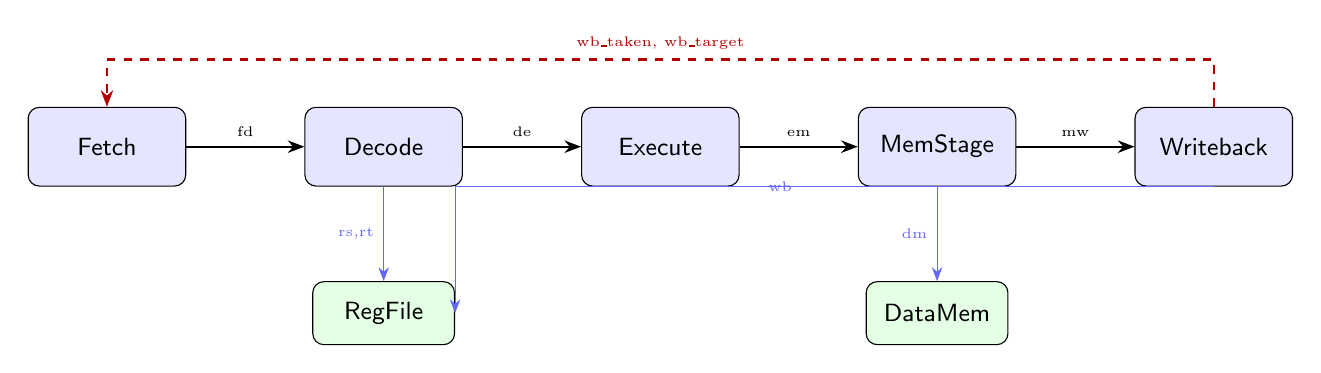
\begin{tikzpicture}[
  stage/.style={draw, rounded corners, minimum width=2cm, minimum height=1cm,
    fill=blue!10, font=\small\sffamily},
  server/.style={draw, rounded corners, minimum width=1.8cm, minimum height=0.8cm,
    fill=green!10, font=\small\sffamily},
  chan/.style={-{Stealth[length=6pt]}, thick},
  feedback/.style={-{Stealth[length=6pt]}, thick, dashed, color=red!70!black},
  req/.style={-{Stealth[length=5pt]}, thin, color=blue!60},
]
  \node[stage] (F) {Fetch};
  \node[stage, right=1.5cm of F] (D) {Decode};
  \node[stage, right=1.5cm of D] (E) {Execute};
  \node[stage, right=1.5cm of E] (M) {MemStage};
  \node[stage, right=1.5cm of M] (W) {Writeback};

  \node[server, below=1.2cm of D] (RF) {RegFile};
  \node[server, below=1.2cm of M] (DM) {DataMem};

  % Pipeline channels
  \draw[chan] (F) -- node[above,font=\tiny] {fd} (D);
  \draw[chan] (D) -- node[above,font=\tiny] {de} (E);
  \draw[chan] (E) -- node[above,font=\tiny] {em} (M);
  \draw[chan] (M) -- node[above,font=\tiny] {mw} (W);

  % Feedback
  \draw[feedback] (W.north) -- ++(0,0.6) -| node[above,font=\tiny,pos=0.25]
    {wb\_taken, wb\_target} (F.north);

  % Server connections
  \draw[req] (D.south) -- node[left,font=\tiny] {rs,rt} (RF.north);
  \draw[req] (W.south) -| node[right,font=\tiny,pos=0.3] {wb} (RF.east);
  \draw[req] (M.south) -- node[left,font=\tiny] {dm} (DM.north);
\end{tikzpicture}
\caption{MiniMIPS pipeline architecture.  Solid arrows: pipeline data flow.
  Dashed arrow: branch feedback from Writeback to Fetch.  Thin arrows:
  server access (request/response).}
\label{fig:pipeline}
\end{figure}

%----------------------------------------------------------------------
\section{Process Implementations}

\subsection{Fetch}

The Fetch process manages the program counter, reads from instruction memory,
and handles branch delay slots.  It loads the program from a hex file at
initialization using the \texttt{readHexInts} intrinsic.

\begin{lstlisting}[style=csp,caption={Fetch process}]
int(32) imem[4096]; int(32) pc;
int(1) fb_taken; int(32) fb_target;
bool in_delay_slot; int(32) delay_target;

count = readHexInts("program.hex", 4096, imem);
pc = 0; in_delay_slot-;

*[ true ->
  instr = imem[pc >> 2];
  fd_pc!pc; fd_instr!instr;
  wb_taken?fb_taken; wb_target?fb_target;
  [ in_delay_slot ->
      pc = delay_target; in_delay_slot-
  [] ~in_delay_slot ->
      [ fb_taken != 0 ->
          delay_target = fb_target;
          in_delay_slot+; pc = pc + 4
      [] else ->
          pc = pc + 4
      ]
  ]
]
\end{lstlisting}

The delay slot mechanism implements the MIPS branch delay slot convention:
when a branch is taken, Fetch executes the next sequential instruction (the
delay slot) before redirecting to the branch target
\cite{Patterson2014,MIPSR3000}.

\subsection{Decode}

Decode extracts instruction fields using shift-and-mask operations and reads
register values from the RegFile server.  It special-cases SYSCALL to read
\texttt{\$v0} and \texttt{\$a0} instead of the instruction's \texttt{rs}/\texttt{rt}
fields.

\begin{lstlisting}[style=csp,caption={Decode process (simplified)}]
*[ true ->
  fd_pc?pc; fd_instr?instr;
  opcode = (instr >> 26) & 0x3F;
  rs = (instr >> 21) & 0x1F;
  rt = (instr >> 16) & 0x1F;
  imm16 = instr & 0xFFFF;
  // Sign-extend
  [ imm16 >= 0x8000 -> imm_sx = 0xFFFF0000 | imm16
  [] else -> imm_sx = imm16
  ];
  // RegFile read (SYSCALL special case)
  [ opcode == 0 & funct == 0x0C ->
      rs_req!2; rs_resp?rs_val;       // $v0
      rt_req!4; rt_resp?rt_val        // $a0
  [] else ->
      rs_req!rs; rs_resp?rs_val;
      rt_req!rt; rt_resp?rt_val
  ];
  de_pc!pc; de_instr!instr;
  de_rs_val!rs_val; de_rt_val!rt_val; de_imm!imm_sx
]
\end{lstlisting}

\subsection{Execute}

Execute is the largest process, implementing all ${\sim}50$ MIPS~I integer
instructions.  It maintains the HI/LO registers internally for
multiply/divide operations.  Selected instruction implementations:

\begin{lstlisting}[style=csp,caption={Execute process (selected instructions)}]
*[ running ->
  de_pc?pc; de_instr?instr;
  de_rs_val?rs_val; de_rt_val?rt_val; de_imm?imm;
  opcode = (instr >> 26) & 0x3F;
  funct = instr & 0x3F;
  result = 0; taken = 0; dest = 0; reg_write = 0;

  [ opcode == 0 ->
    [ funct == 0x21 ->                  // ADDU
        result = (rs_val + rt_val) & 0xFFFFFFFF;
        dest = rd; reg_write = 1
    [] funct == 0x00 ->                 // SLL
        result = (rt_val << shamt) & 0xFFFFFFFF;
        dest = rd; reg_write = 1
    [] funct == 0x2A ->                 // SLT (signed)
        [ rs_val >= 0x80000000 & rt_val < 0x80000000 ->
            result = 1
        [] rs_val < 0x80000000 & rt_val >= 0x80000000 ->
            result = 0
        [] rs_val < rt_val -> result = 1
        [] else -> result = 0
        ];
        dest = rd; reg_write = 1
    [] funct == 0x18 ->                 // MULT
        prod = rs_val * rt_val;
        lo = prod & 0xFFFFFFFF;
        hi = (prod >> 32) & 0xFFFFFFFF
    [] funct == 0x0C ->                 // SYSCALL
        [ rs_val == 1 -> print("" + rt_val)
        [] rs_val == 10 -> print("HALT"); running-
        [] else -> skip
        ]
    // ... (remaining R-type instructions)
    ]
  [] opcode == 4 ->                     // BEQ
      branch_target = pc + 4 + (imm << 2);
      [ rs_val == rt_val -> taken = 1
      [] else -> taken = 0
      ]
  [] opcode == 3 ->                     // JAL
      branch_target = ((pc+4) & 0xF0000000)
                    | (jtarget << 2);
      taken = 1; result = pc + 8;
      dest = 31; reg_write = 1
  [] opcode == 0x23 ->                  // LW
      result = (rs_val + imm) & 0xFFFFFFFF;
      memop = 5; dest = rt; reg_write = 1
  [] opcode == 0x2B ->                  // SW
      result = (rs_val + imm) & 0xFFFFFFFF;
      store_data = rt_val; memop = 8
  // ... (remaining I-type and J-type)
  ];
  em_result!result; em_store_data!store_data;
  em_dest!dest; em_rw!reg_write; em_memop!memop;
  em_taken!taken; em_target!branch_target
]
\end{lstlisting}

\subsection{RegFile Server}

The register file is a \emph{server process}---it does not initiate
communication but responds to requests.  In each cycle it serves two reads
(from Decode) and one conditional write (from Writeback), in a fixed order
that matches the pipeline sequencing:

\begin{lstlisting}[style=csp,caption={Register file server}]
int(32) reg[32];
int(5) rn; int(1) wen; int(5) wreg; int(32) wval;

*[ true ->
  rs_req?rn; rs_resp!reg[rn];          // read rs
  rt_req?rn; rt_resp!reg[rn];          // read rt
  wb_wen?wen; wb_wreg?wreg; wb_wval?wval;
  #[ wen != 0 & wreg != 0 -> reg[wreg] = wval ]
]
\end{lstlisting}

The guarded command \texttt{\#[~\ldots~]} is an \emph{optional} execution:
the body executes only if the guard is true.  Register \texttt{\$0} is
hardwired to zero by the guard \texttt{wreg~$\neq$~0}.

\subsection{DataMem Server}

The data memory server handles byte, halfword, and word access in
little-endian byte order:

\begin{lstlisting}[style=csp,caption={Data memory server (selected operations)}]
int(8) mem[65536];
int(4) op; int(32) addr; int(32) wdata; int(32) result;

*[ true ->
  dm_op?op; dm_addr?addr; dm_wdata?wdata;
  [ op == 5 ->                          // LW
      a = addr & 0xFFFC;
      result = (mem[a+3] << 24) | (mem[a+2] << 16)
             | (mem[a+1] << 8) | mem[a]
  [] op == 8 ->                         // SW
      a = addr & 0xFFFC;
      mem[a] = wdata & 0xFF;
      mem[a+1] = (wdata >> 8) & 0xFF;
      mem[a+2] = (wdata >> 16) & 0xFF;
      mem[a+3] = (wdata >> 24) & 0xFF;
      result = 0
  // ... (LB, LBU, LH, LHU, SB, SH)
  ];
  dm_rdata!result
]
\end{lstlisting}

%----------------------------------------------------------------------
\section{System Composition}

The seven processes are composed in parallel and connected through named
channels using the system description language.  The \texttt{.sys} file
declares channels with explicit bit widths and binds process ports to
channels:

\begin{lstlisting}[style=csp,caption={System description (abbreviated)}]
system MiniMIPS;
  var fd_pc    : channel(32);
  var fd_instr : channel(32);
  var de_pc    : channel(32);
  // ... (30 channels total)

  process Fetch    = "fetch.csp"    port out fd_pc ...;
  process Decode   = "decode.csp"   port in  fd_pc ...;
  process Execute  = "execute.csp"  port in  de_pc ...;
  process MemStage = "memstage.csp" port in  em_result ...;
  process Writeback= "writeback.csp"port in  mw_result ...;
  process RegFile  = "regfile.csp"  port in  rs_req ...;
  process DataMem  = "dmem.csp"     port in  dm_op ...;
begin
  var fetch : Fetch(fd_pc => fd_pc, ...);
  // ... (7 process instances)
end.
\end{lstlisting}

%----------------------------------------------------------------------
\section{Correctness Argument}

The decomposition preserves correctness because:

\begin{enumerate}
\item Each pipeline stage performs exactly the computation that the sequential
  specification performs at the corresponding phase.  The channel
  communications enforce the ordering: Decode cannot proceed until Fetch has
  sent, Execute cannot proceed until Decode has sent, etc.

\item The sequential pipeline (one instruction in flight at a time) means there
  are no data hazards, control hazards, or structural hazards.  Writeback
  completes and writes to the register file before the next instruction's
  Decode reads from it.

\item The branch delay slot is handled at the Fetch level: when a taken branch
  is detected, Fetch executes the delay slot instruction at PC+4 before
  jumping to the branch target.  This matches the MIPS architectural
  specification \cite{MIPSR3000,Patterson2014}.

\item Register \texttt{\$0} is protected: the RegFile server refuses writes to
  register~0, maintaining the invariant that \texttt{reg[0]~=~0}.
\end{enumerate}

\subsection{Verification by Simulation}

We verified the implementation by executing hand-assembled MIPS programs
through the CSP simulator generated by the cspbuild tool chain.  The test
suite covers:

\begin{table}[ht]
\centering
\begin{tabular}{@{}lll@{}}
\toprule
Test & Instructions exercised & Expected output \\
\midrule
\texttt{trivial} & ADDIU, SYSCALL & 42, HALT \\
\texttt{arith}   & ADDU, SUBU, SLL, SRL, AND, OR, XOR, SLTU &
  15, 7, 44, 22, 0, 15, 15, 1, HALT \\
\texttt{branch}  & BEQ, BNE, J, delay slots & 10, 20, 99, HALT \\
\texttt{loop}    & BEQ (loop), ADDIU, ADDU & 15 (= $\sum_{i=1}^{5} i$), HALT \\
\texttt{memory}  & SW, LW & 42, 100, HALT \\
\texttt{jal}     & JAL, JR, delay slots & 7 (= 3+4), HALT \\
\bottomrule
\end{tabular}
\caption{Test programs and results.  All tests produce the expected output.}
\label{tab:tests}
\end{table}

%----------------------------------------------------------------------
\section{Implementation Notes}

\subsection{Toolchain}

The implementation uses the following tool chain:
\begin{itemize}
\item \textbf{cspfe}: CSP frontend parser (Modula-3), converts \texttt{.csp}
  source to S-expression intermediate form.
\item \textbf{cspc}: CSP compiler (Scheme/mscheme), performs optimization
  passes and generates Modula-3 simulation code.
\item \textbf{cspbuild}: System builder (Scheme), parses \texttt{.sys} files,
  compiles each process, generates harness, and invokes cm3 (Modula-3
  compiler) to produce the simulator binary.
\item \textbf{cm3}: Critical Mass Modula-3 compiler, compiles generated
  Modula-3 to native code.
\end{itemize}

\subsection{CSP Language Features Used}

\begin{itemize}
\item \texttt{int(N)}: unsigned $N$-bit integer type.  For $N \leq 63$ on
  64-bit platforms, these map to native machine integers; wider types use
  arbitrary-precision arithmetic.

\item \texttt{chan!expr} / \texttt{chan?var}: channel send and receive.
  These are blocking synchronous operations (rendezvous).

\item \texttt{*[~guard~$\to$~body~]}: infinite loop with guard.

\item \texttt{\#[~guard~$\to$~body~]}: optional execution (executes body
  only if guard is true).

\item \texttt{[~g1~$\to$~s1~$\square$~g2~$\to$~s2~]}: deterministic
  selection (if-else).

\item \texttt{readHexInts(path, max, array)}: built-in intrinsic that loads
  hexadecimal integers from a file into an array.
\end{itemize}

\subsection{Compiler Extensions}

Two extensions were made to the CSP compiler to support this project:

\begin{enumerate}
\item \textbf{\texttt{readHexInts} intrinsic}: Added to the simulation
  runtime (\texttt{CspIntrinsics.m3}) and code generator
  (\texttt{codegen-m3.scm}) to enable loading programs from hex files at
  simulation startup.

\item \textbf{Native left-shift code generation}: The code generator's
  handling of the \texttt{<<} operator for native integer types was missing;
  it fell through to the arbitrary-precision path.  Added a case to generate
  \texttt{Word.Shift} for native types.
\end{enumerate}

%----------------------------------------------------------------------
\section{Related Work}

The original MiniMIPS processor was designed at Caltech by Alain Martin's
research group \cite{MiniMIPS2002,Lines1998}.  It was a full asynchronous
implementation of the MIPS R3000, fabricated in 0.18\textmu m CMOS, and
demonstrated competitive performance with synchronous designs of the same era.
Our work is a software-level reimplementation of the same architectural concept,
targeting simulation rather than silicon.

Martin's synthesis methodology is described in detail in
\cite{Martin1990,Martin2006,MartinSynthesis}.  The key insight is that CSP
channel communication provides both data transfer and synchronization, allowing
systematic decomposition of sequential computations into concurrent processes.

Hoare's original CSP formalism \cite{Hoare1978,Hoare1985} provides the
theoretical foundation.  The adaptation of CSP for VLSI design is described in
\cite{Martin1990}, with extensions for production rules and handshaking
protocols.

The MIPS instruction set architecture is documented in \cite{MIPSR3000} and
explained pedagogically in \cite{Patterson2014}.  Our implementation covers
the complete MIPS~I user-mode integer instruction set, excluding floating-point
and privileged (CP0) instructions.

The async-toolkit \cite{AsyncToolkit} provides the CSP compiler
infrastructure used in this work.  It includes the cspfe parser, cspc compiler,
and cspbuild system builder.

%----------------------------------------------------------------------
\section{Conclusion}

We have presented MiniMIPS, a complete MIPS~I user-mode processor implemented
as a network of seven communicating sequential processes.  The design follows
Martin's synthesis methodology, beginning from a sequential specification and
decomposing into concurrent pipeline stages.  All arithmetic, logic, shift,
branch, jump, load/store, multiply/divide, and system call instructions are
implemented and verified through simulation with hand-assembled test programs.

The implementation demonstrates that the CSP-based hardware description
approach scales to realistic processor designs, and that the cspbuild tool
chain can compile and simulate complex multi-process systems.

\begin{thebibliography}{99}

\bibitem[Martin(1990)]{Martin1990}
A.~J. Martin.
\newblock Programming in VLSI: From communicating processes to delay-insensitive
  circuits.
\newblock In C.~A.~R. Hoare, editor, \emph{Developments in Concurrency and
  Communication}, UT Year of Programming Series, pages 1--64. Addison-Wesley,
  1990.

\bibitem[Martin(2006)]{Martin2006}
A.~J. Martin and M.~Nystr\"om.
\newblock Asynchronous techniques for system-on-chip design.
\newblock \emph{Proceedings of the IEEE}, 94(6):1089--1120, 2006.

\bibitem[Martin et~al.(1997)]{MartinSynthesis}
A.~J. Martin, A.~Lines, R.~Manohar, M.~Nystr\"om, P.~Penzes, R.~Southworth,
  U.~Cummings, and T.~K. Lee.
\newblock The design of an asynchronous MIPS R3000 microprocessor.
\newblock In \emph{Proceedings of the 17th Conference on Advanced Research in
  VLSI (ARVLSI)}, pages 164--181, 1997.

\bibitem[Lines(1998)]{Lines1998}
A.~Lines.
\newblock Pipelined asynchronous circuits.
\newblock Master's thesis, California Institute of Technology, 1998.

\bibitem[Martin et~al.(2002)]{MiniMIPS2002}
A.~J. Martin, M.~Nystr\"om, and P.~Penzes.
\newblock \emph{Et2: A Metric for Time and Energy Efficiency of Computation}.
\newblock In R.~Madhavan and D.~Madhavan, editors, \emph{Power Aware Design
  Methodologies}, pages 141--173. Kluwer, 2002.

\bibitem[Hoare(1978)]{Hoare1978}
C.~A.~R. Hoare.
\newblock Communicating sequential processes.
\newblock \emph{Communications of the ACM}, 21(8):666--677, 1978.

\bibitem[Hoare(1985)]{Hoare1985}
C.~A.~R. Hoare.
\newblock \emph{Communicating Sequential Processes}.
\newblock Prentice Hall, 1985.

\bibitem[Patterson and Hennessy(2014)]{Patterson2014}
D.~A. Patterson and J.~L. Hennessy.
\newblock \emph{Computer Organization and Design: The Hardware/Software
  Interface}.
\newblock Morgan Kaufmann, 5th edition, 2014.

\bibitem[MIPS(1991)]{MIPSR3000}
MIPS Computer Systems.
\newblock \emph{MIPS R3000 RISC Processor User's Manual}.
\newblock 1991.

\bibitem[Intel Labs(2024)]{AsyncToolkit}
Intel Labs.
\newblock Async-toolkit: Asynchronous circuit design CAD tools.
\newblock \url{https://github.com/IntelLabs/async-toolkit}, 2024.

\end{thebibliography}

\end{document}
